\documentclass[journal]{IEEEtran}
\usepackage{amsmath,amssymb,amsfonts}
\usepackage{algorithm}
\usepackage{array}
\usepackage[caption=false,font=normalsize,labelfont=sf,textfont=sf]{subfig}
\usepackage{textcomp}
\usepackage{stfloats}
\usepackage{url}
\usepackage{verbatim}
\usepackage{graphicx}
\usepackage{cite}
\usepackage{graphicx,color}
\usepackage{tcolorbox}
\usepackage{orcidlink}
\usepackage{tikz}
\usepackage{algpseudocode}
\usepackage{pgfplots}
\usepackage{float}
\pgfplotsset{compat=1.17}
\usetikzlibrary{positioning}
\usetikzlibrary{calc}
\hyphenation{op-tical net-works semi-conduc-tor IEEE-Xplore}
\providecommand{\authorrefmark}[1]{\textsuperscript{#1}}
% updated with editorial comments 8/9/2021

\begin{document}

\title{Energy theft probability classification with adaptive observation windows in a digital twin for NB-IoT forensic telemetry}

\author{
J. D. S. Coutinho Filho\authorrefmark{1,2,4} \orcidlink{0009-0005-5972-7962},
C. Marcon\authorrefmark{3} \orcidlink{0000-0002-7811-7896}, J. A. N. da Silveira\authorrefmark{1,2} \orcidlink{0000-0003-2590-9520},
\\
R. G. Diógenes Filho\authorrefmark{4} \orcidlink{0009-0007-5461-7937},
M. E. Matos\authorrefmark{5} \orcidlink{0009-0003-3098-3239}
%
\thanks{\authorrefmark{1}Department of Teleinformatics Engineering, Fortaleza, Brazil.}
\thanks{\authorrefmark{2}Federal University of Ceará (UFC), Fortaleza, Brazil.}
\thanks{\authorrefmark{3}Pontifical Catholic University of Rio Grande do Sul (PUCRS), Porto Alegre, Brazil.}
\thanks{\authorrefmark{4}Center of Studies and Research of the North and Northeast (NEPEN), Fortaleza, Brazil.}
\thanks{\authorrefmark{5}EDP South America, São José dos Campos, Brazil.}
\thanks{Corresponding author: J. D. S. Coutinho Filho, \\e-mail:            danilocoutinho@lesc.ufc.br.}
\thanks{This work was supported in part by the Coordenação de Aperfeiçoamento de Pessoal de Nível Superior (CAPES), Brazil---Finance Code 001, and by the Programa de Excelência Acadêmica (PROEX).}
\thanks{Manuscript received April 29, 2026; revised XX XX, 2026.}
}


% The paper headers
\markboth{IEEE Journal on Selected Areas in Communications,~Vol.~XX, No.~XX, April~2026}%
{Coutinho Filho\MakeLowercase{\textit{et al.}}: Energy theft probability classification with adaptive observation windows in a digital twin for NB-IoT forensic telemetry}

\IEEEpubid{0000--0000/00\$00.00~\copyright~2026 IEEE}
% Remember, if you use this you must call \IEEEpubidadjcol in the second
% column for its text to clear the IEEEpubid mark.

\maketitle

\begin{abstract}
Non-technical losses remain a major challenge for electric power distribution utilities, particularly because suspicious behaviors are often intermittent, making fixed-rate telemetry either insufficient for forensic analysis or inefficient in terms of communication cost. This paper proposes a digital-twin-driven framework that treats telemetry density as a controllable resource and adapts observation windows based on contextual theft-risk estimation. The proposed system integrates forensic and billing data, applies interpretable and supervised risk models, and dynamically reconfigures NB-IoT telemetry in a closed loop. Experimental results across six controlled scenarios show that the adaptive policy preserves up to 97\% of the detection performance of dense monitoring while reducing communication volume by more than 50\%. These results demonstrate that digital twins can effectively optimize forensic observability in communication-constrained smart metering systems. 
\end{abstract}

\begin{IEEEkeywords}
Digital twin, non-technical losses, energy theft detection, adaptive telemetry, closed-loop optimization.
\end{IEEEkeywords}

\section{Introduction}
\IEEEPARstart{T}{he} non-technical losses (NTLs) remain a significant challenge for power distribution utilities, regulators, and sector operators. Among their most recurrent causes are energy theft, partial or selective bypass, meter tampering, and other fraudulent consumption mechanisms that directly affect revenue collection and the reliability of operational supervision. In practice, such behaviors tend to occur at specific times of day or under particular operating conditions, rather than continuously. This temporal selectivity makes conventional fixed-period monitoring strategies intrinsically limited for forensic purposes.

At low acquisition rates, relevant evidence may not be captured when suspicious behavior occurs, whereas maintaining permanently high sampling and transmission rates imposes communication and processing costs disproportionate to the operational benefit during normal operation. Thus, the central challenge is not only to classify theft risk from telemetry, but also to determine when increasing the temporal resolution of observations is technically justified.

Although the literature on NTL detection has reported increasingly robust classification results using smart meter and Advanced Metering Infrastructure (AMI) data, most approaches inherently assume fixed-cadence measurement streams and focus on improving classification within a predefined observation process \cite{b2,b4,b5,b6}. In parallel, digital-twin studies for smart metering have predominantly emphasized virtualization and monitoring, rather than application-oriented control of the sensing process \cite{b19,b20,b22}. Similarly, adaptive telemetry methods in IoT and LPWAN systems have largely focused on bandwidth or energy efficiency, without explicitly linking sensing density to the forensic value of the observed context \cite{b26,b27,b29}. As a result, an important gap remains at the intersection of these research lines: the lack of a closed-loop framework in which a digital twin integrates contextual evidence and dynamically adapts observation density based on its expected forensic utility. This gap motivates the central hypothesis of this work: An application-oriented digital twin can use contextual theft-risk estimates to adapt the observation window of NarrowBand Internet of Things (NB-IoT) forensic telemetry, thereby preserving most of the detection performance associated with dense monitoring while substantially reducing communication costs. Under this formulation, risk estimation is treated as a control signal that governs the observation process, reframing the problem from static classification toward application-oriented closed-loop optimization.

In this work, the digital twin is defined as an application-oriented software entity capable of maintaining contextual state, integrating heterogeneous measurements, estimating the probability of theft, and feeding the result back into the telemetry-configuration process. In this sense, the twin acts as a decision layer that converts contextual evidence into sensing actions, consistent with the broader view of digital twins as closed-loop cyber-physical mechanisms for monitoring, prediction, and adaptive control \cite{b15,b16,b24}. \IEEEpubidadjcol

The system considered in this paper consists of a dedicated forensic telemetry device installed in parallel with the billing meter, using NB-IoT as the primary communication technology and Bluetooth Low Energy (BLE) as a local contingency channel. It is assumed that the embedded layer already provides instantaneous electrical quantities, historical profiles, alarms, local persistence, and configurable telemetry parameters. The main contribution of this study lies in the software layer of the digital twin, which combines billing and inspection measurements, derives contextual features, estimates the probability of theft, and governs a closed-loop adaptive observation-window policy.

Fig.~\ref{fig:use_case_topology} summarizes the physical and logical topology considered in this work, highlighting the placement of the inspection meter on the utility service branch, its relationship to the billing meter, and the telemetry flow toward the analytics platform.

\begin{figure}[t]
    \centering
    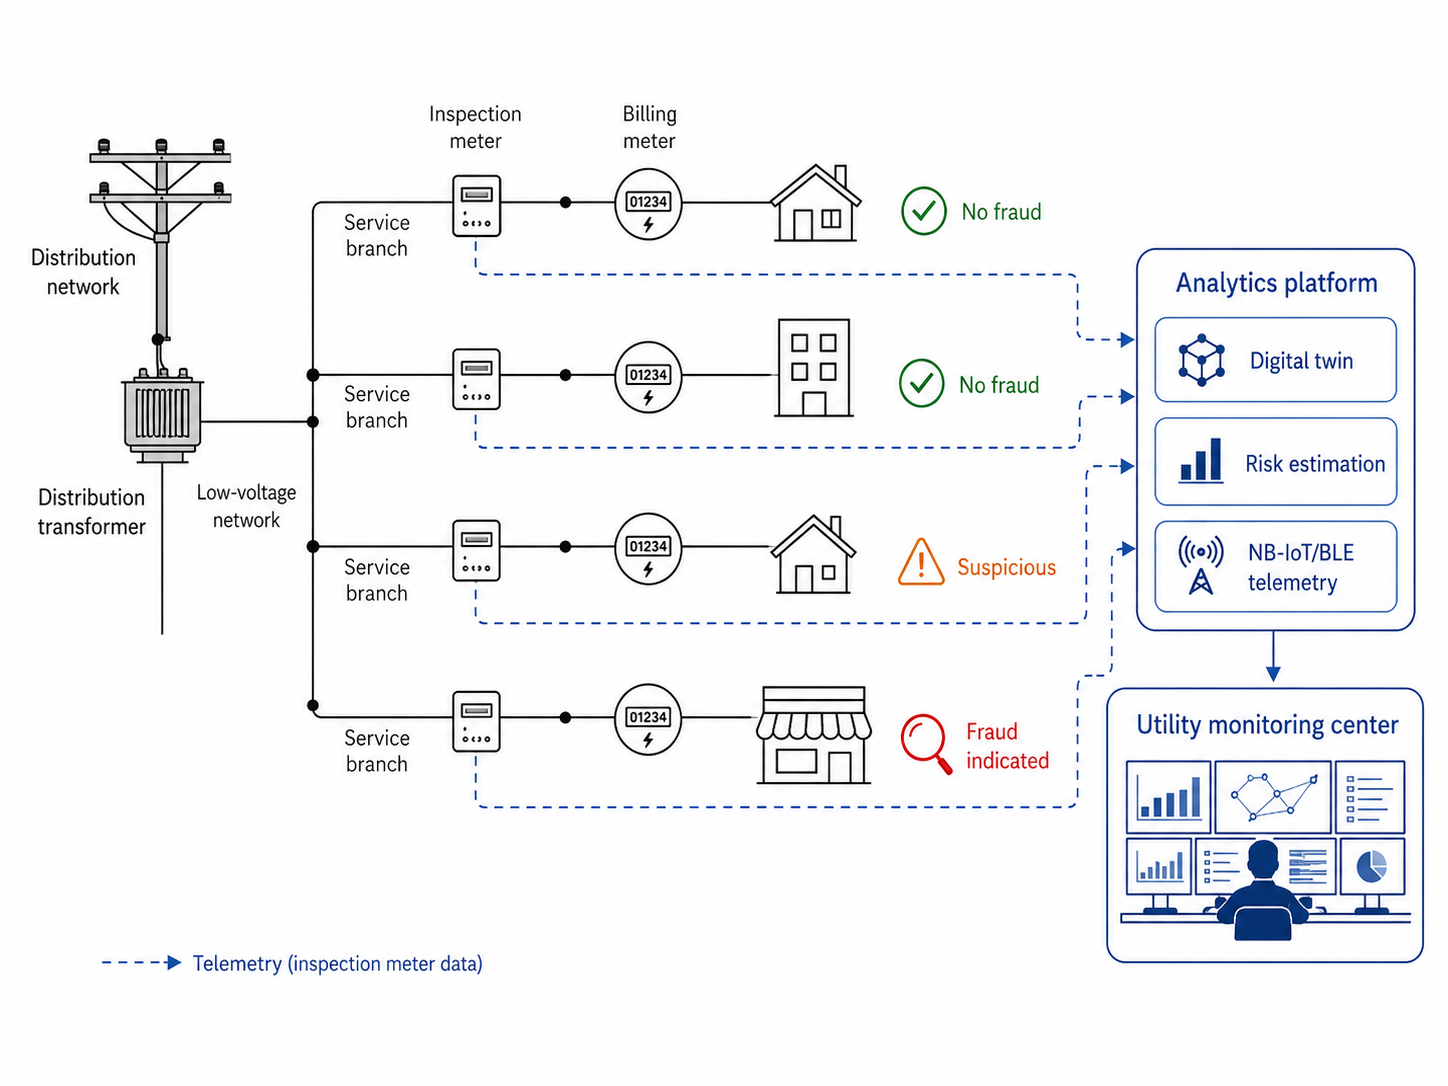
\includegraphics[width=\columnwidth]{fig/topologia_artigo.png}
    \caption{Simplified use-case topology of the proposed forensic telemetry framework.}
    \label{fig:use_case_topology}
\end{figure}

The main contributions of this work are fourfold:
\begin{itemize}
    \item to formulate energy-theft monitoring as a closed-loop observation-control problem, in which telemetry density is treated as a controllable resource rather than as a fixed input to classification;
    \item to design and implement an application-oriented digital twin for forensic energy telemetry, grounded on a real firmware-level device and capable of fusing billing and inspection data into contextual theft-risk estimates;
    \item to propose an adaptive observation-window policy that reconfigures the capture interval according to the estimated risk, thus enabling risk-triggered densification of NB-IoT telemetry; and
    \item to provide a fully reproducible multi-scenario experimental campaign for comparing fixed and adaptive policies under both detection and communication-cost metrics.
\end{itemize}

The remainder of this paper is organized as follows. Section~\ref{sec:related_work} situates the work within the literature and makes explicit the research gap it addresses. Section~\ref{sec:Materials_Methods} presents the system model and main assumptions, and describes the proposed framework, including the reproducible prototype architecture, the contextual risk model, the observation policies, and the experimental methodology. Section ~\ref{sec:Results_Discussion} presents and discusses the results, including an analysis of limitations and possible extensions. Finally, Section~\ref{sec:Conclusion} concludes the paper.

\section{RELATED WORK} \label{sec:related_work}
This section reviews the most relevant literature related to the problem addressed in this paper, focusing on three axes: (i) energy theft and NTL detection in smart metering, (ii) the use of digital twins in smart metering and cyber-physical monitoring, and (iii) adaptive telemetry under communication constraints. Rather than providing a purely descriptive overview, this section aims to situate the present work relative to the closest studies and to clarify which capabilities are already available in the literature and which combinations remain insufficiently explored.


\subsection{Bibliographic Search Strategy and Study Selection}
The related literature was identified through a structured search in major databases (IEEE Xplore, Springer, ScienceDirect, and MDPI), covering publications from 2019 to 2025, with updates through March 2026. The search strategy was designed to cover the three central components of the problem investigated in this paper: energy-theft detection, digital-twin-based monitoring, and adaptive telemetry.

The search was guided by the following three complementary queries:
\begin{itemize}
    \item \textit{\textbf{Query A --- Energy theft and non-technical-loss detection:} (``energy theft OR ``electricity theft" OR ``non-technical loss*" OR NTL OR fraud OR tamper*) AND (``smart meter*" OR ``advanced metering infrastructure" OR AMI) AND (detect* OR classif* OR anomal* OR ``machine learning" OR ``deep learning")}
    \item \textit{\textbf{Query B --- Digital twins for smart metering and energy monitoring:} (``digital twin*" OR ``cyber-physical" OR ``virtual replica") AND (``smart meter*" OR ``smart grid" OR ``power distribution" OR ``energy monitoring") AND (monitor* OR anomaly OR fault OR secur* OR telemetry OR ``real-time")}
    \item \textit{\textbf{Query C --- Adaptive telemetry and communication-efficient monitoring:} (("NB-IoT" OR "narrowband IoT" OR LPWAN OR BLE OR telemetry OR "remote metering") AND ("smart meter*" OR "energy meter*" OR "forensic telemetry") AND (adaptive OR dynamic OR "observation window*" OR "sampling rate" OR "transmission interval" OR reconfigur* OR "closed-loop"))}
\end{itemize}

%\begin{tcolorbox}[colback=white, colframe=black, boxrule=0.2pt, width=1.0\columnwidth, arc=0mm, auto outer arc]
%\textit{\textbf{Query A --- Energy theft and non-technical-loss detection:} ("energy theft" OR "electricity theft" OR "non-technical loss*" OR NTL OR fraud OR tamper*) AND ("smart meter*" OR "advanced metering infrastructure" OR AMI) AND (detect* OR classif* OR anomal* OR "machine learning" OR "deep learning")}
%\end{tcolorbox}
%\label{qA}

%\begin{tcolorbox}[colback=white, colframe=black, boxrule=0.2pt, width=1.0\columnwidth, arc=0mm, auto outer arc]
%\textit{\textbf{Query B --- Digital twins for smart metering and energy monitoring:} ("digital twin*" OR "cyber-physical" OR "virtual replica") AND ("smart meter*" OR "smart grid" OR "power distribution" OR "energy monitoring") AND (monitor* OR anomaly OR fault OR secur* OR telemetry OR "real-time")}
%\end{tcolorbox}
%\label{qB}

%\begin{tcolorbox}[colback=white, colframe=black, boxrule=0.2pt, width=1.0\columnwidth, arc=0mm, auto outer arc]
%\textit{\textbf{Query C --- Adaptive telemetry and communication-efficient monitoring:} (("NB-IoT" OR "narrowband IoT" OR LPWAN OR BLE OR telemetry OR "remote metering") AND ("smart meter*" OR "energy meter*" OR "forensic telemetry") AND (adaptive OR dynamic OR "observation window*" OR "sampling rate" OR "transmission interval" OR reconfigur* OR "closed-loop"))}
%\end{tcolorbox}
%\label{qC}

The queries were applied, with minor syntactic adaptations, across the different bibliographic databases. The initial retrieval yielded 91 records. After duplicate removal, 78 records remained. Screening by title, abstract, and keywords reduced this set to 42 studies; full-text review yielded a final core set of 31 works discussed in this section.

As inclusion criteria, studies were retained if they presented at least one of the following aspects: (i) methods for energy-theft or non-technical-loss detection using smart meter or AMI data; (ii) digital-twin-based approaches for smart metering, smart grids, or energy monitoring; or (iii) adaptive telemetry, sensing, or communication strategies relevant to NB-IoT, LPWAN, or resource-constrained IoT monitoring. Exclusion criteria removed generic works on IoT, smart cities, or digital twins that had no direct relation to smart metering, energy monitoring, or adaptive observation, as well as studies whose contributions were distant from the forensic telemetry problem addressed in this paper.

Rather than being a full systematic review, this procedure should be interpreted as a structured, reproducible bibliographic selection protocol aimed at technically positioning the present study. The resulting corpus was organized into three groups corresponding to the main research lines discussed next.

\subsection{Energy-Theft and Non-Technical-Loss Detection from Smart Metering Data}
The detection of NTLs and the identification of energy theft have been extensively investigated using data collected from smart meters and AMI. Previous studies have shown that supervised machine learning, deep learning, and ensemble-based methods can detect suspicious consumption behavior with good classification performance when historical load series are available \cite{b1, b2, b3, b4, b5, b6}.

This body of literature has evolved from conventional classifiers to more sophisticated architectures designed to address class imbalance, temporal variation, and attack diversity. CNN-based, CNN-LSTM, transformer-based, and stacked-ensemble models have been proposed to improve discrimination between legitimate and malicious users, while one-class and zero-day approaches seek to generalize to previously unseen fraud patterns \cite{b7, b8, b9, b10, b11, b12}. Other studies have incorporated clustering strategies, feeder-level aggregation, or contextual customer modeling to reduce false positives and increase robustness to heterogeneous consumption profiles \cite{b13, b14}.

Despite these advances, the dominant assumption in most NTL studies is that telemetry is already available at a fixed cadence. As a consequence, prior work has focused on improving classification under a predefined observation process, rather than questioning whether the observation process itself should be dynamically adapted to the forensic relevance of the current context \cite{b2, b5, b6}.


\subsection{Digital Twins for Smart Metering and Cyber-Physical Monitoring}
In parallel with research on energy-theft detection, digital twins have emerged as an important paradigm for cyber-physical monitoring, prediction, and decision support. In general terms, a digital twin maintains a synchronized virtual representation of a physical asset or process and exploits this representation for monitoring, fault analysis, simulation, and operational guidance \cite{b15, b16, b17}. In energy-related domains, digital twins have been applied to smart-meter virtualization, real-time monitoring, predictive analysis, communication-aware services, and secure integration of IoT-based systems \cite{b18, b19, b20, b21, b22}.

In the context of smart metering, existing digital-twin studies emphasize the virtualization of meter functions, bidirectional communication between the device and the cloud, and the use of real-time monitoring dashboards that support operational services and remote interaction \cite{b19, b20, b22}. More broadly, the digital-twin literature highlights closed-loop monitoring, predictive maintenance, and adaptive control as central properties of mature cyber-physical deployments \cite{b23, b24, b25}. However, in smart metering, the twin is still used predominantly for representation, supervision, and service support, rather than as an application-oriented decision layer that can reallocate sensing effort based on contextual value \cite{b18, b20, b22}. This limits the role of digital twins to passive monitoring, leaving unexplored their potential as active sensing and control entities.

\subsection{Adaptive Telemetry and the Still-Unresolved Intersection}
A third body of literature addresses adaptive telemetry, communication-efficient monitoring, and anomaly detection in IoT and industrial systems. These studies show that dynamic transmission policies, adaptive anomaly detection, and edge-assisted intelligence can reduce bandwidth or energy consumption while preserving monitoring capability \cite{b26, b27, b28}. In smart-metering and LPWAN scenarios, adaptive algorithms have also been proposed to adjust transmission intervals based on the observed dynamics of sensed data, yielding significant savings in packet volume and communication-related energy costs, including in NB-IoT environments \cite{b29}. Related NB-IoT smart-metering work also reinforces the feasibility of lightweight, long-range telemetry for remote measurement and distributed configuration \cite{b30, b31}.

These adaptive-telemetry studies usually optimize communication efficiency for generic monitoring objectives rather than for application-oriented tasks such as distinguishing theft from non-theft conditions. In contrast, energy-theft detection studies typically optimize classification accuracy while assuming a fixed observation process, whereas digital-twin studies in smart metering rarely turn observation density itself into a decision-controlled variable. This leaves open the combination of contextual theft-risk estimation, digital-twin-based decision support, and adaptive observation under communication constraints \cite{b6, b14, b22, b29}.

The present study is positioned at this intersection. Rather than treating telemetry cadence as fixed, it models sensing density as a controllable resource and uses the digital twin as a closed-loop decision layer for risk-driven forensic observability in LPWAN-based telemetry, specifically using NB-IoT.

\subsection{Comparative Summary}

\begin{table*}[!ht]
\centering
\caption{Positioning of this work relative to the closest literature}
\label{tab:rw_comparison}
\begin{tabular}{|p{2cm}|p{4.6cm}|p{2.4cm}|p{4.1cm}|p{1.9cm}|}
\hline
\textbf{Research line} & \textbf{Core contribution} & \textbf{Typical assumption} & \textbf{Main limitation} & \textbf{Representative references} \\
\hline
Energy theft / NTL detection & Theft detection from smart meter or AMI data using ML, DL, ensembles, or anomaly models & Fixed-cadence telemetry & Does not treat observation density as a control variable & \cite{b1,b2,b3,b4,b5,b6,b7,b8,b9,b10,b11,b12,b13,b14} \\
\hline
Digital twins for smart metering & Virtualization, synchronized monitoring, remote interaction, and operational support & Twin used mainly for supervision or services & Rarely uses the twin as an application-aware sensing control layer & \cite{b18,b19,b20,b21,b22,b23,b24,b25} \\
\hline
Adaptive telemetry / communication-efficient monitoring & Dynamic reporting for bandwidth or energy reduction & Efficiency-driven adaptation & Does not optimize telemetry for theft-oriented forensic utility & \cite{b26,b27,b28,b29,b30,b31} \\
\hline
This work & Contextual theft-risk estimation with digital-twin-guided adaptive observation for NB-IoT forensic telemetry & Observation density is controllable & Balances detection capability and communication cost & This article \\
\hline
\end{tabular}
\end{table*}

Table~\ref{tab:rw_comparison} summarizes the positioning of the present work with respect to the three closest lines of literature. In summary, prior literature provides important foundations in three complementary directions: energy-theft detection from smart meter data, the use of digital twins for monitoring and decision support, and adaptive telemetry in communication-constrained IoT systems. However, these components remain only weakly articulated in the context of forensic observability in electrical metering systems. The main gap, therefore, is the lack of frameworks that explicitly treat observation density as a controllable resource and leverage digital twins as decision layers to allocate sensing effort based on contextual forensic value.

\section{MATERIALS AND METHODS} \label{sec:Materials_Methods}
\subsection{Methodological Overview}

\begin{comment}
    architecture figure
    flowchart LR

  subgraph PR["Physical and Runtime Layer"]
    direction LR
    SPT["Synthetic physical timeline"]
    MBM["MockBillingMeter"]
    SR["SimulationRunner"]
    MFD["MockForensicDevice"]

    SPT --> SR
    MBM --> SR
  end

  subgraph DT["Digital Twin Layer"]
    direction LR
    TO["TwinObservation"]
    FT["ForensicTwin"]
    TSS["TwinStateSnapshot"]

    TO --> FT
    FT --> TSS
  end

  subgraph DL["Decision Layer"]
    direction LR
    DE["DecisionEngine"]
    PF["Probability fusion"]

    DE --> PF
  end

  subgraph PL["Policy Layer"]
    direction LR
    PO["PolicyOrchestrator"]
    TRD["TelemetryReconfigurationDecision"]

    PO --> TRD
  end

  subgraph CD["Command Delivery Layer"]
    direction LR
    MT["MockTransport<br/>NB-IoT / BLE"]
  end

  subgraph PRR["Persistence and Reproducibility Layer"]
    direction LR
    LOGS["State history, decisions,<br/>command plan, <br/>transport logs,<br/>manifests and reports"]
  end

  SR --> TO
  FT --> DE
  PF --> PO
  TRD --> MT

  MT -->|delivered command reconfigures emission gate| MFD
  MFD --> SR
  MT -->|delivered command updates twin state| FT

  TSS --> LOGS
  TRD --> LOGS
  MT --> LOGS
\end{comment}

This section describes the experimental framework implemented to evaluate energy-theft probability classification with adaptive observation control in an NB-IoT-based forensic telemetry scenario. The methodological objective is not merely to estimate risk from previously available telemetry, but to materialize an application-oriented digital twin capable of interpreting context, determining observation density, and locally updating the capture regime throughout the experimental execution.

The framework was built as a reproducible local-execution prototype, fully implemented in Python, with simplified installation, SQLite persistence, and command-line execution. This design choice had two main motivations. First, it ensured that the experiments reported in the paper could be reproduced without mandatory dependence on external infrastructure. Second, it allowed the digital-twin architecture to be made explicit in code before integration with real data, an NB-IoT broker, and real-time BLE contingency.

% Optimized from original paragraph 3: reduced repetition around “framework”, “implementation”, and “closed loop”.
Conceptually, the framework is organized into six layers: data ingestion, contextual enrichment, risk engines, explicit digital-twin state, policy orchestration, and local closed-loop runtime with simulated devices. Unlike a static classification pipeline, the current implementation contains explicit entities for twin state, decision, command plan, and execution of the perception--decision--action cycle.


\subsection{System Under Consideration and Firmware-Integration Assumptions}
The target system consists of a billing meter and a discrete forensic telemetry device installed in parallel with the monitored installation. It is assumed that the embedded layer already provides, through the existing firmware, instantaneous electrical quantities, historical profiles, alarms, local persistence, and telemetry parameters remotely configurable via NB-IoT, with BLE available as a local contingency channel.

At this stage of the study, integration with the physical layer was represented by synthetic traces semantically aligned with the firmware domain. The field names used in data generation and processing preserve this semantic proximity without breaking the logical architecture of the framework, including: `voltage\_rms', `current\_rms', `active\_power', `reactive\_power', `apparent\_power', `power\_factor', `active\_energy', `reactive\_energy', `alarm\_overvoltage', `alarm\_undervoltage', `alarm\_overcurrent', and `alarm\_out\_of\_bounds\_power'.


\subsection{Implemented Digital-Twin Architecture}
The core of the framework is the \textit{ForensicTwin} digital twin, implemented as a software entity with its own state and event-oriented updates. At each observed event, the twin receives a \textit{TwinObservation}, produced from the temporal fusion of forensic measurements, billing measurements, and alarm events. This observation contains the electrical, temporal, operational, and alarm-related attributes required for risk inference.

A \textit{DecisionEngine} operates on this observational state and is responsible for transforming the current context into a probabilistic risk decision. The engine uses two evidence sources: a rule-based contextual baseline and a supervised logistic-regression baseline. Rather than assuming a single fixed combination rule, the framework was extended to support three explicit probability-fusion strategies: \textit{weighted}, \textit{conservative\_max}, and \textit{context\_aware}. This choice allows fusion to be treated as an experimental methodological variable rather than as a hidden implementation detail.

The output of the \textit{DecisionEngine} is consumed by a \textit{PolicyOrchestrator}, which converts the decision into an observational action. This action is formalized in the \textit{TelemetryReconfigurationDecision} structure, which represents the command plan issued by the digital twin. Among other fields, the command specifies the monitored asset identifier, the selected mode, the capture interval, the decision probability, the probability source, the textual justification, and the preferred transport.

To materialize the closed loop in a local environment, the framework further uses three simulation components: \textit{MockForensicDevice}, \textit{MockBillingMeter}, and \textit{MockTransport}. The first simulates the forensic device and adjusts its future emission cadence based on the received command. The second provides the billing reference. The third simulates local command delivery, with preferential use of NB-IoT and fallback to BLE in degraded scenarios (which, in a real system, would require a local operator with a BLE-enabled device). The integrated execution of these components is handled by \textit{SimulationRunner}, which explicitly implements the framework's local closed loop.

\begin{figure*}[!t]
      \centering
      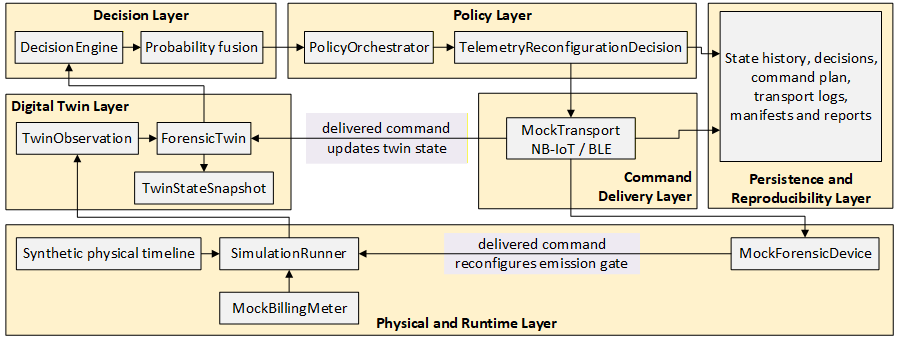
\includegraphics[width=0.9\textwidth]{fig/framework_architecture2.png}
      \caption{Closed-loop architecture of the proposed digital-twin framework.}
      \label{fig:framework_architecture}
\end{figure*}

The implemented framework architecture is summarized in Fig.~\ref{fig:framework_architecture}. As shown, the core of the system is composed of the \textit{ForensicTwin}, the decision layer \textit{DecisionEngine}, the policy-orchestration layer \textit{PolicyOrchestrator}, and the explicit command-plan formalization \textit{TelemetryReconfigurationDecision}. These components operate jointly with the local runtime and the simulated devices, materializing a closed loop in which the twin's decision changes the future observation density.


\subsection{Problem Formulation} \label{subsec:problem_formulation}
The problem investigated in this work can be formulated as an adaptive observation-control problem in forensic telemetry. At each potential acquisition instant, the system has access to an observational state summarizing the electrical, temporal, operational, and historical conditions of the monitored asset. Based on this state, the digital twin must decide which observation regime to apply to the forensic device to balance the capability for detecting suspicious behavior and communication costs.

Let $s_t$ denote the system state at time $t$, composed of attributes derived from forensic measurement, billing measurement, temporal context, alarm context, and operational link integrity. In the current prototype, $s_t$ includes, among other variables, relative power divergence, accumulated energy difference, moving averages of divergence, hourly recurrence, alarm score, \textit{link}, and \textit{heartbeat}.

The action $a_t$ chosen by the digital twin corresponds to the observation mode to be applied after evaluation of the current state. In the proposed framework, the action space is discrete and given by
\[
\mathcal{A} = \{\text{basal},\, \text{moderate},\, \text{aggressive}\},
\]
where each action induces a distinct capture interval. In the implemented prototype, these modes correspond to acquisition intervals of 60, 15, and 5 minutes, respectively.

The system dynamics are partially controlled because the action taken at time $t$ alters the future observation density, thereby changing the information available at subsequent times. This property distinguishes the problem from static classification over a fixed sample set: the decision policy affects the observation process that will feed future decisions. This behavior reinforces that observation density is effectively treated as a controllable variable rather than a fixed parameter.

The objective of the digital twin is to select a sequence of actions $\{a_t\}$ that maximizes the forensic utility of observation under communication-cost constraints. Conceptually, this objective can be written as
\[
\max_{\{a_t\}} \; U = \lambda_1 \cdot D - \lambda_2 \cdot C,
\]
where $D$ denotes suspicious-behavior detection capability and $C$ denotes the communication cost induced by the observation policy. The coefficients $\lambda_1$ and $\lambda_2$ express the relative importance of forensic sensitivity and communication efficiency.

Since the above utility is not directly observable, the paper adopts experimental metrics that approximate it. The detection component is evaluated using precision, recall, F1-score, and critical-slot hit rate, whereas the cost component is approximated primarily by communication volume in bytes. In addition, the false-alert rate serves as an auxiliary metric for assessing the operational burden of more aggressive observation regimes.

Under this formulation, the problem solved by the framework is not merely to classify theft versus non-theft, but to decide when it is worthwhile to increase the temporal resolution of observation. In other words, the risk probability estimated by the twin engines is treated as a control signal governing telemetry density, rather than merely as the final output of a classifier.


\subsection{Formalization of the Local Closed Loop}
The local runtime executes the following cycle in temporal order:

\begin{enumerate}
    \item traverses the synthetic physical timeline at native resolution;
    \item checks, through the \textit{MockForensicDevice}, whether the current event should be emitted according to the active capture interval;
    \item whenever the event is emitted, constructs a \textit{TwinObservation};
    \item evaluates the observation with the \textit{DecisionEngine};
    \item applies a probabilistic fusion strategy;
    \item generates a \textit{TelemetryReconfigurationDecision} with the \textit{PolicyOrchestrator};
    \item delivers the command through the \textit{MockTransport};
    \item applies the command to the \textit{ForensicTwin} and to the \textit{MockForensicDevice}; and
    \item updates the twin state and the future emission cadence.
\end{enumerate}

Algorithm~\ref{alg:closed_loop_twin} illustrates the above cycle. This modeling choice is important because it shifts the experiment from a simple offline evaluation on fixed samples to an environment in which observability itself becomes a consequence of the twins' decisions. Although the physical loop is local and simulated, the logical structure of perception, inference, action, and feedback is already explicitly materialized.

\begin{algorithm}[!ht]
\caption{Local closed loop of the digital twin}
\label{alg:closed_loop_twin}
\begin{algorithmic}[1]
\Require Synthetic timeline $\mathcal{X}$, twin $T$, forensic device $D$, billing meter $B$, transport $L$
\ForAll{instant $x_t \in \mathcal{X}$}
    \If{$D.\text{should\_emit}(x_t)$}
        \State $o_t \gets \text{build\_observation}(x_t, B)$
        \State $d_t \gets T.\text{update}(o_t)$
        \State $c_t \gets \text{PolicyOrchestrator}(d_t)$
        \State $L.\text{deliver}(c_t)$
        \State $T.\text{apply}(c_t)$
        \State $D.\text{apply}(c_t)$
    \EndIf
\EndFor
\end{algorithmic}
\end{algorithm}


\subsection{Feature Construction and Risk Engines}
Risk features were constructed from four evidence groups, all derived from a synthetic stream designed to preserve metrological coherence among RMS voltage ($V$), RMS current ($I$), active power ($P$), reactive power ($Q$), apparent power ($S$), power factor, and accumulated energies. In particular, the synthetic scenarios were not generated as an independent series of electrical variables, but as traces in which instantaneous and accumulated quantities remain physically compatible. This choice ensures that the risk features extracted by the framework correspond to electrically plausible observational discrepancies, rather than to arbitrary differences between artificial time series.

The first feature group corresponds to the electrical divergence between the forensic and billing measurements. This class includes quantities such as relative active-power divergence, accumulated active-energy difference, moving averages of divergence, and moving maxima over short windows. Since both measurement streams preserve internal consistency among $V$, $I$, $P$, $Q$, and $S$, the divergence observed between the forensic device and the billing meter can be interpreted as a metrological discrepancy consistent with hypotheses of theft or selective under-registration. In other words, the framework does not compare only two active-power series, but rather two electrically consistent descriptions of the same observed process from distinct perspectives.

The second group corresponds to the temporal context. It includes features such as hour of day, day of week, and historical recurrence of suspicious divergence within the same time slot. This layer is relevant because many theft behaviors do not manifest continuously, but rather within selective windows, such as peak periods or recurrent nighttime intervals. Thus, risk depends not only on the instantaneous magnitude of divergence, but also on its temporal repetition within specific operational intervals.

The third group corresponds to alarm context, with aggregation of events such as out-of-bounds power, overcurrent, undervoltage, and overvoltage. In the current synthetic generator, these alarms are derived directly from the simulated electrical quantities and therefore remain semantically consistent with the system's physical state. This allows the decision layer to use alarms not as independent artificial labels but as complementary evidence that is coherent with the underlying electrical dynamics.

The fourth group comprises operational signals such as link integrity and \textit{heartbeat}. These attributes are used to distinguish low observability caused by communication degradation from a genuinely suspicious electrical context. This separation is methodologically important because it prevents absence or sparsity of data from being automatically interpreted as evidence of theft.

Two risk engines operate on this feature set. The first is a rule-based baseline designed for auditability and interpretability. This engine explicitly combines divergence magnitude, temporal persistence, alarm context, and operational integrity to produce a comprehensible and traceable risk score. The second is a supervised baseline based on logistic regression, with numerical preprocessing and explicit \textit{fallback} for single-class scenarios in the training split. At this stage, the supervised baseline is not intended to maximize predictive complexity, but rather to provide a second explainable probability source for the twins' decision layer.


\subsection{Probability-Fusion Strategies} \label{subsec:fusao}
\begin{table}[ht]
\centering
\caption{Legend of the mathematical symbols used in the probability-fusion formulation.}
\label{tab:fusion_symbols}
\begin{tabular}{p{1.3cm} p{6.38cm}}
\hline
\textbf{Symbol} & \textbf{Meaning} \\
\hline
$t$ & Temporal index of the observed event \\
$p_t^{(r)}$ & Risk probability estimated by the rule-based engine at time $t$ \\
$p_t^{(s)}$ & Risk probability estimated by the supervised engine at time $t$ \\
$p_t^{(d)}$ & Final probability used by the digital-twin decision layer at time $t$ \\
$\alpha$ & Weight assigned to the rule-based component in the \textit{weighted} strategy \\
$1-\alpha$ & Weight assigned to the supervised component in the \textit{weighted} strategy \\
$\mathcal{C}_t$ & Observational context at time $t$, composed of electrical, temporal, operational, and alarm evidence \\
$w_r(\mathcal{C}_t)$ & Contextual weight assigned to the rule-based engine in the \textit{context\_aware} strategy \\
$w_s(\mathcal{C}_t)$ & Contextual weight assigned to the supervised engine in the \textit{context\_aware} strategy \\
$\max(\cdot)$ & Maximum operator, used to select the highest probability among two sources \\
\hline
\end{tabular}
\end{table}

Let $p_t^{(r)} \in [0,1]$ denote the risk probability estimated by the rule-based engine at time $t$, and let $p_t^{(s)} \in [0,1]$ denote the probability estimated by the supervised baseline. The purpose of the fusion layer is to produce a single decision probability,
\[
 p_t^{(d)} \in [0,1],
\]
which the digital twin will use as the control signal to select the subsequent observation regime.

Three fusion strategies were considered.

In the \textit{weighted} strategy, the decision probability is given by a convex combination of the two evidence sources:
\[
 p_t^{(d)} = w_r \, p_t^{(r)} + w_s \, p_t^{(s)},
\]
with
\[
 w_r + w_s = 1, \qquad w_r, w_s \geq 0.
\]
In the current prototype, $w_r > w_s$ is adopted so as to favor the interpretability and robustness of the rule-based component without discarding the additional information provided by the supervised baseline.

In the \textit{conservative\_max} strategy, the probabilistic decision is defined as
\[
 p_t^{(d)} = \max\left(p_t^{(r)},\, p_t^{(s)}\right).
\]
This policy corresponds to a conservative stance for inspection purposes, in which the final decision inherits the highest risk indication among the two sources. Operationally, this strategy tends to increase system sensitivity, at the potential cost of denser observations and higher communication volume.

In the \textit{context\_aware} strategy, the fusion weights depend on the electrical and operational context observed at time $t$. Let $c_t$ denote a categorical context variable such that
\[
 c_t \in \{\text{electrical-dominant},\, \text{temporal-dominant},\, \text{balanced}\}.
\]
The final probability is then written as
\[
 p_t^{(d)} = w_r(c_t) \, p_t^{(r)} + w_s(c_t) \, p_t^{(s)},
\]
with
\[
 w_r(c_t) + w_s(c_t) = 1.
\]
In the implemented prototype, the contextual rule can be summarized as follows:
\[
 c_t =
\begin{cases}
\text{electrical-dominant}, &
\parbox[t]{\linewidth}{\raggedright
if active alarms are present or \\
electrical divergence is strong,}\\
\text{temporal-dominant}, &
\parbox[t]{\linewidth}{\raggedright
if relevant temporal recurrence \\
is present without dominant \\
electrical evidence,}\\
\text{balanced}, &
\text{otherwise}.
\end{cases}
\]
When $c_t = \text{electrical-dominant}$, greater weight is assigned to the rule-based engine; when $c_t = \text{temporal-dominant}$, the influence of the supervised component is increased; and, in the balanced case, an intermediate combination is used. This formulation allows the decision layer to adapt the fusion process based on the predominant type of evidence available at each instant.

\begin{table*}[ht]
\centering
\caption{Comparison of the probability-fusion strategies considered in the framework.}
\label{tab:fusion_strategies}
\begin{tabular}{p{2.0cm} p{4.2cm} p{4.4cm} p{4.6cm}}
\hline
\textbf{Strategy} & \textbf{Mathematical definition} & \textbf{Operational interpretation} & \textbf{Main methodological risk} \\
\hline
\textit{weighted} & $p_t^{(d)} = \alpha p_t^{(r)} + (1-\alpha)p_t^{(s)}$, with $\alpha \in [0,1]$ and greater weight assigned to the rule-based component & Robust compromise in terms of average sensitivity, balancing interpretability and generalization without exclusively privileging a single source & May excessively smooth critical evidence if the weights are poorly calibrated, thereby reducing sensitivity to short or highly localized events \\
\textit{conservative\_max} & $p_t^{(d)} = \max\{p_t^{(r)}, p_t^{(s)}\}$ & Conservative inspection-oriented policy, prioritizing the highest suspicion available among the two sources & Tends to increase sensitivity at the cost of higher false-alert rates and higher communication cost due to more frequent densification \\
\textit{context\_aware} & $p_t^{(d)} = w_r(\mathcal{C}_t)p_t^{(r)} + w_s(\mathcal{C}_t)p_t^{(s)}$, with $w_r(\mathcal{C}_t)+w_s(\mathcal{C}_t)=1$ and weights defined by the observational context & Semantic adaptation to the type of evidence, prioritizing alarms and strong electrical signals or, alternatively, temporal recurrence and historical patterns & Depends on the quality of contextual modeling; if the weight-switching rules are poorly specified, it may introduce interpretability instability or decision bias \\
\hline
\end{tabular}
\end{table*}

The introduction of this fusion layer addresses a limitation of the initial prototype, in which the adaptive policy relied exclusively on the rule-based score. Under the current formulation, the observation policy becomes governed by a decision variable explicitly built from multiple evidence sources, making fusion part of the experimental method rather than merely an implementation detail.

Tables~\ref{tab:fusion_symbols} and~\ref{tab:fusion_strategies} complement this formulation by summarizing the symbols used in the fusion layer and the methodological differences among the three strategies considered, respectively.


\subsection{Synthetic Data Generation and Scenarios}
The experimental campaign was built upon six controlled synthetic scenarios: normal operation, persistent theft, peak-hour theft, nighttime theft, intermittent nighttime theft, and disturbance without theft. Each scenario covers seven days of observation at a native 15-minute resolution. Generation was implemented deterministically, with explicit random seeds, producing three temporal streams per scenario: forensic-device measurements, billing-meter measurements, and alarm events.

Unlike purely statistical generation, the synthetic traces were structured to preserve metrological coherence among voltage, current, active power, reactive power, apparent power, power factor, and accumulated energies. At each interval, RMS voltage and active power are first defined from the scenario load profile, after which the power factor is sampled within a plausible range and used to consistently derive apparent power, reactive power, and RMS current. Active and reactive energies are then accumulated over time according to the 15-minute time step, preserving consistency between instantaneous quantities and integrated consumption.

The discrepancy between the forensic meter and the billing meter arises from a theft ratio that depends on the scenario and the temporal instant. When a theft event is active, the billing meter's measured active power is lower than that observed by the forensic device. From this new power value, the full set of billing meter quantities is recalculated in an internally consistent manner, including RMS current, apparent power, reactive power, power factor, and accumulated energy. In this way, the synthetic scenario preserves the physical assumption that the forensic device observes higher consumption than that effectively recorded for billing, without violating the fundamental relationships among the electrical variables.

Synthetic alarms are also derived from the system's electrical and operational states. Events such as overvoltage, undervoltage, overcurrent, and out-of-bounds power are generated by applying thresholds to the simulated quantities, whereas operational-integrity signals such as \textit{link} and \textit{heartbeat} are produced to represent communication degradation. Thus, the scenarios provide a controlled environment for jointly evaluating electrical divergence, temporal recurrence, alarm context, and operational effects on the adaptive observation policy.

This strategy does not replace validation with field data, but it provides a reproducible and physically more consistent experimental environment for evaluating framework coherence, closed-loop dynamics, and the trade-offs among observation policies.

Fig.~\ref{fig:experimental_methodology} summarizes the methodological flow adopted in the framework evaluation. Synthetic scenarios are used as input to a local closed runtime in which the digital twin estimates risk, governs the observation policy, and generates reconfiguration decisions. From this execution, the metrics and artifacts that support the comparative analysis of observation regimes and the study of the trade-off between detection capability and communication cost are obtained.

\begin{figure}[!ht]
    \centering
    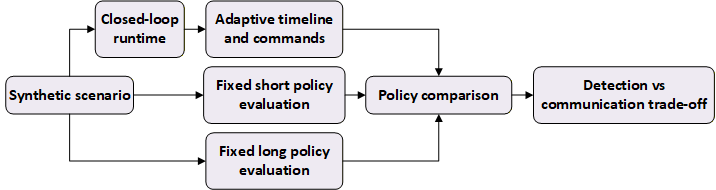
\includegraphics[width=\columnwidth]{fig/experimental_methodology2.png}
    \caption{Workflow of the comparative evaluation of the proposed framework.}
    \label{fig:experimental_methodology}
\end{figure}


\subsection{Metrics, Traceability, and Reproducibility}
Framework evaluation was conducted with metrics that reflect not only classification performance, but also the operational utility of the closed-loop observation policy. For this purpose, the metrics were organized into three groups: detection capability, communication cost, and forensic utility of observation.

\begin{comment}
\begin{table*}[!ht]
\centering
\caption{Methodological interpretation of the metrics used in framework evaluation.}
\label{tab:evaluation_metrics}
\begin{tabular}{p{2.4cm} p{2.1cm} p{5.0cm} p{5.0cm}}
\hline
\textbf{Metric} & \textbf{Type} & \textbf{Interpretation in the problem} & \textbf{Risk of isolated optimization} \\
\hline
Precision & Detection & Measures the proportion of events classified as suspicious that actually correspond to theft or anomalous behavior & May induce excessively conservative policies, reducing sensitivity to short or intermittent events \\
\textit{Recall} & Detection & Measures the ability to cover effectively suspicious events, particularly relevant in temporally selective fraud & May increase communication cost and false-alert rate if optimized without control \\
F1-score & Aggregate detection & Summarizes the trade-off between precision and \textit{recall}, favoring global policy comparison & May conceal important operational differences when policies have very distinct costs \\
Communication bytes & Operational cost & Approximates the main policy cost, since higher capture density implies larger transmitted volume & May favor overly economical policies that miss critical observation windows \\
Critical slot hit & Forensic utility & Indicates whether the policy observed the time interval of greatest forensic interest, capturing the temporal value of evidence & Does not replace aggregate metrics; a policy may hit the critical window and still exhibit low overall quality \\
False alert rate & Operational risk & Measures the frequency of undue suspicion, relevant for containing unnecessary densification and improper inspection escalation & If optimized in isolation, may excessively reduce system sensitivity to real suspicious behavior \\
\hline
\end{tabular}
\end{table*}
\end{comment}

The first group includes precision, recall, and F1-score. Precision indicates the proportion of events classified as suspicious that actually correspond to anomalous behavior, and is therefore relevant for limiting unnecessary intensification of observation. Recall measures the system's ability to cover effectively suspicious events, a particularly important aspect in intermittent or temporally selective fraud. F1-score was adopted as a compromise measure between precision and recall, providing a more balanced view of performance in the presence of asymmetric distributions of normal and suspicious events.

The second group captures the operational cost of the policy, approximated mainly by total communication volume in bytes. This choice follows from the fact that, in the proposed framework, the control variable is observation density, which directly translates into more or less transmitted volume. In NB-IoT-based scenarios, this metric serves as a natural proxy for communication cost, since it synthesizes the joint effect of capture frequency, transmission frequency, and the temporal persistence of denser observation modes.

The third group comprises two metrics related to forensic utility and operational risk. The first is \textit{critical slot hit}, which indicates whether the policy was able to adequately observe the time interval of greatest forensic interest in the analyzed scenario. This metric is especially relevant in this work because the central hypothesis is not merely to detect anomalies on average, but to selectively densify observations precisely during periods when suspicious behavior is more likely to occur. The second is the false-alert rate, which quantifies the proportion of events or intervals classified as suspicious that do not correspond to actual theft. In an inspection context, this metric is relevant because false alerts affect not only the statistical quality of inference but may also induce additional communication costs, unnecessarily dense observation, and undue escalation of investigative actions.

Beyond aggregate metrics, the framework generates structured traceability artifacts, including twin-state history, issued decisions, command plans, transport-delivery logs, and execution manifests. These artifacts serve two complementary methodological roles: they enable detailed auditing of the digital twin's internal behavior throughout execution, and they directly connect the experimental results to the narrative elements reported in the paper, thereby strengthening the reproducibility and verifiability of the empirical evidence presented.

Table~\ref{tab:evaluation_metrics} complements the experimental formulation by making explicit the role of each metric in the studied problem, as well as the methodological risks associated with isolated optimization.

\begin{table}[!ht]
\centering
\caption{Summary of the evaluation metrics.}
\label{tab:evaluation_metrics}
\scriptsize
\begin{tabular}{p{2.35cm} p{2.25cm} c}
\hline
\textbf{Metric} & \textbf{Type} & \textbf{Note} \\
\hline
Precision & Detection & 1 \\
\textit{Recall} & Detection & 2 \\
F1-score & Aggregate detection & 3 \\
Communication bytes & Operational cost & 4 \\
Critical slot hit & Forensic utility & 5 \\
False-alert rate & Operational risk & 6 \\
\hline
\end{tabular}

\vspace{0.5mm}
\begin{minipage}{\columnwidth}
\footnotesize
1: Measures the fraction of suspicious classifications that correspond to actual theft or anomalies; isolated optimization may reduce sensitivity\\
2: Measures coverage of suspicious events, especially temporally selective fraud; isolated optimization may increase cost and false alerts\\
3: Summarizes the trade-off between precision and \textit{recall}; it may mask operational differences among policies with distinct costs\\
4: Approximates policy cost via transmitted volume; isolated optimization may favor policies that miss critical windows\\
5: Indicates whether the most relevant forensic interval was observed; it does not replace aggregate metrics\\
6: Measures undue suspicion and escalation risk; isolated optimization may reduce sensitivity to real anomalies
\end{minipage}
\end{table}

\section{RESULTS AND DISCUSSION}  \label{sec:Results_Discussion}
This section presents and analyzes the results obtained from the complete execution of the proposed framework. The discussion emphasizes the digital twin's behavior as a closed-loop adaptive-observation mechanism and demonstrates its ability to balance detection capability and communication cost across multiple scenarios.


\subsection{Evidence of Closed-Loop Digital-Twin Execution}
The first relevant evidence is not yet classificatory, but architectural and operational. In the reference execution reported in this work, carried out over a deterministic seven-day synthetic scenario with fixed seed, the runtime traversed 672 potential acquisition instances and effectively observed 231 samples under the default adaptive policy with \textit{weighted} fusion. In this same execution, 45 reconfiguration commands were issued, and 12 transport fallback events from NB-IoT to BLE were recorded. The modal distribution of the observation regime was also asymmetric and semantically consistent with the expected framework behavior: 588 instants remained in \textit{basal} mode, 28 in \textit{moderate} mode, and 56 in \textit{aggressive} mode.

This evidence is important because it demonstrates that the \textit{ForensicTwin}, the \textit{DecisionEngine}, the \textit{PolicyOrchestrator}, the \textit{MockTransport}, and the \textit{MockForensicDevice} were exercised as coupled components of a closed-loop architecture. In other words, the results presented below do not derive merely from \textit{a posteriori} resampling over a fixed dataset, but from a runtime in which the observation process itself depends on the policy decided by the digital twin.


\subsection{Aggregate Performance of Observation Policies}
\begin{comment}
\begin{table*}[ht]
\centering
\caption{Aggregate comparison of the main observation policies.}
\label{tab:agg_policy_results}
\begin{tabular}{p{1.5cm} p{3.0cm} p{2.0cm} p{2.0cm} p{2.4cm} p{3.7cm}}
\hline
\textbf{Policy} & \textbf{Probability source/fusion} & \textbf{F1-score} & \textbf{Recall} & \textbf{Communication bytes} & \textbf{Interpretation} \\
\hline
\textit{adaptive} & \textit{decision\_probability} / \textit{weighted} & 0.6468 & 0.6307 & 18{,}848 & Preserves most of the dense-monitoring benefit with substantially lower communication cost \\
\textit{fixed\_short} & supervised probability & 0.6667 & 0.6667 & 43{,}008 & Highest aggregate detection performance, but at the highest communication cost \\
\textit{fixed\_long} & supervised probability & 0.2556 & 0.1583 & 10{,}752 & Lowest communication cost, but severe under-observation and poor recall \\
\hline
\end{tabular}
\end{table*} 
\end{comment}

The aggregate comparison across policies confirms the central hypothesis of this work: the adaptive policy preserves over 97\% of the detection performance of dense monitoring while reducing communication cost by more than 56\%. Considering the main adaptive configuration, namely the \textit{adaptive} policy governed by \textit{decision\_probability} with \textit{weighted} fusion, the framework achieved an average F1-score of 0.6468, an average \textit{recall} of 0.6307, and an average communication volume of 18{,}848 bytes across the six evaluated scenarios.

As shown in Table~\ref{tab:agg_policy_results}, when compared with the \textit{fixed\_short} policy based on supervised probability, which achieved an average F1-score of 0.6667, \textit{recall} of 0.6667, and a cost of 43{,}008 bytes, the adaptive policy preserved approximately 97.0\% of aggregate F1 and 94.6\% of \textit{recall}, while reducing communication volume by approximately 56.2\%. This result demonstrates that high-resolution monitoring is not required continuously, but can be selectively activated based on contextual risk without significant loss in detection performance.


\begin{table}[ht]
\centering
\caption{Summary of the main observation policies.}
\label{tab:agg_policy_results}
\scriptsize
\begin{tabular}{lcccc c}
\hline
\textbf{Policy} & \textbf{Source/fusion} & \textbf{F1} & \textbf{Rec.} & \textbf{Bytes} & \textbf{Note} \\
\hline
\textit{adaptive} 
& DP / W 
& 0.6468 & 0.6307 & 18,848 & 1 \\

\textit{fixed-short} 
& Sup. 
& 0.6667 & 0.6667 & 43,008 & 2 \\

\textit{fixed-long} 
& Sup. 
& 0.2556 & 0.1583 & 10,752 & 3 \\
\hline
\end{tabular}

\vspace{0.5mm}
\begin{minipage}{\columnwidth}
\footnotesize
1: Dense-monitoring benefit with substantially lower communication cost\\
2: Highest detection performance, but at the highest communication cost\\
3: Lowest communication cost, but with under-observation and poor recall
\end{minipage}
\end{table}

Comparison with the \textit{fixed\_long} policy reinforces this interpretation from another perspective. The \textit{fixed\_long} policy based on supervised probability used only 10{,}752 bytes, but with an average \textit{recall} of 0.1583 and an F1-score of 0.2556. Hence, the gain of the adaptive policy is not only absolute in F1, but also qualitative: it occupies an effective intermediate regime between an extreme economy and permanent dense monitoring. Operationally, this means that the digital twin avoided both the ongoing cost of short fixed telemetry and the severe under-observation associated with the long fixed policy.


\subsection{Scenario-Level Analysis}
The scenario-level analysis shows that the benefit of adaptation is not uniform, but strongly depends on the temporal structure of suspicious behavior.

In the \textit{persistent\_theft} scenario, the adaptive policy achieved performance equivalent to that of the fixed short policy. In all relevant variants, the system observed 672 samples, used 43{,}008 bytes, and achieved precision, \textit{recall}, and F1-score all equal to 1.0. This behavior confirms that, under persistent suspicious conditions, the adaptive policy naturally converges to dense monitoring, effectively reproducing the fixed short regime.

The selective-in-time theft scenarios were more informative. In \textit{peak\_theft}, the adaptive policy with \textit{weighted} fusion observed 252 samples, consumed 16{,}128 bytes, and achieved an F1-score of 0.9955, compared with 43{,}008 bytes and an F1-score of 1.0 for the supervised fixed short policy. This represents an approximately 62.5\% reduction in communication cost with a practically negligible loss in classification performance. In \textit{night\_theft}, the same pattern was observed: the adaptive policy observed 273 samples, used 17{,}472 bytes, and achieved an F1-score of 0.9964, again remaining very close to the fixed short policy while reducing transmitted volume by approximately 59.4\%.

The \textit{intermittent\_evening} scenario was the most challenging and, for this reason, the most useful for discussing framework limitations. In this case, the adaptive policy with \textit{weighted} fusion observed 234 samples, consumed 14{,}976 bytes, and achieved an F1-score of 0.8889, whereas the supervised fixed short policy achieved an F1-score of 1.0 with 43{,}008 bytes. Thus, even in the most difficult scenario, adaptation preserved good performance at approximately 65.2\% less communication. However, \textit{critical slot hit} remained equal to 0 because the policy observed the critical period with a one-slot temporal displacement, producing a prediction of slot 20 instead of slot 18. This result highlights both a strength and a limitation of the framework: on the one hand, the digital twin concentrated observation around the suspicious region; on the other hand, the binary critical-slot metric strongly penalized a relatively small temporal misalignment.

In the scenarios without effective theft, namely \textit{normal} and \textit{disturbance\_without\_theft}, all policies exhibited stable behavior, with a null F1-score due to the absence of the positive class and a false-alert rate equal to zero. More important than the trivial value of the detection metrics is that the adaptive policy remained economically well-behaved, observing only 168 samples and maintaining a cost of 10{,}752 bytes, equivalent to the fixed long regime. This suggests that the framework does not spuriously intensify observation when contextual evidence does not support a suspicion of theft.


\subsection{Comparison of Fusion Strategies}

% Optimized from original subsection: reduced repetition between “behavior consistent” and detailed interpretation.
The aggregate analysis of fusion strategies indicates that the framework's decision component also behaves consistently. As reported in Table~\ref{tab:agg_fusion_results}, the \textit{weighted} strategy achieved the best average F1-score among the adaptive approaches based on \textit{decision\_probability}, with a value of 0.6468, average \textit{recall} of 0.6307, and communication cost of 18{,}848 bytes. The \textit{context\_aware} strategy remained very close, with an average F1-score of 0.6445 and the same average communication cost. In contrast, the \textit{conservative\_max} strategy achieved a lower average F1-score of 0.5931, a \textit{recall} of 0.6041, a slightly higher cost of 19{,}093 bytes, and a higher aggregate false-alert rate of approximately 0.0106.

\begin{comment}
\begin{table*}[ht]
\centering
\caption{Aggregate comparison of the adaptive probability-fusion strategies.}
\label{tab:agg_fusion_results}
\begin{tabular}{p{2.0cm} p{1.5cm} p{1.5cm} p{2.0cm} p{2.0cm} p{4.0cm}}
\hline
\textbf{Fusion strategy} & \textbf{F1-score} & \textbf{Recall} & \textbf{Communication bytes} & \textbf{False-alert rate} & \textbf{Interpretation} \\
\hline
\textit{weighted} & 0.6468 & 0.6307 & 18{,}848 & 0.0000 & Best average compromise among adaptive strategies \\
\textit{context\_aware} & 0.6445 & 0.6262 & 18{,}848 & 0.0000 & Competitive performance, but still dependent on contextual-model quality \\
\textit{conservative\_max} & 0.5931 & 0.6041 & 19{,}093 & $\approx 0.0106$ & More conservative behavior, with higher densification and more undue suspicion \\
\hline
\end{tabular}
\end{table*}
\end{comment}

\begin{table}[ht]
\centering
\caption{Summary of adaptive probability-fusion strategies.}
\label{tab:agg_fusion_results}
\scriptsize
\begin{tabular}{lcccc c}
\hline
\textbf{Strategy} & \textbf{F1} & \textbf{Rec.} & \textbf{Bytes} & \textbf{FAR} & \textbf{Note} \\
\hline
\textit{weighted} 
& 0.6468 & 0.6307 & 18,848 & 0.0000 & 1 \\

\textit{context-aware} 
& 0.6445 & 0.6262 & 18,848 & 0.0000 & 2 \\

\textit{conservative-max} 
& 0.5931 & 0.6041 & 19,093 & $\approx$0.0106 & 3 \\
\hline
\end{tabular}

\vspace{0.5mm}
\begin{minipage}{\columnwidth}
\footnotesize
1: Best average compromise among adaptive strategies\\
2: Competitive performance, but still dependent on contextual-model quality\\
3: Conservative behavior, with higher density and more undue suspicion
\end{minipage}
\end{table}


These results suggest that the conservative maximum-based stance, although intuitively attractive for inspection purposes, tends to over-amplify isolated evidence, inducing more observational densification than necessary without translating that increase into an average performance gain. By contrast, \textit{weighted} fusion proved to be a robust compromise among interpretability, sensitivity, and cost, while \textit{context\_aware} showed competitive potential but still depends on the quality of the contextual modeling used to modulate the weights.

Overall, these results indicate that balanced fusion strategies are more suitable for adaptive observation control than purely conservative approaches.


\subsection{Critical Assessment of the Adopted Metrics}
The selected metrics proved useful in capturing distinct dimensions of the problem. F1-score was the most informative aggregate measure for comparing observation regimes in scenarios with and without suspicious events. Communication volume in bytes served as an adequate operational proxy for cost, since the experiment was designed to precisely assess the effect of observation density on communication load. The false-alert rate was also informative, particularly in showing that the \textit{conservative\_max} strategy produced a small but non-negligible increase in undue suspicion.

The \textit{critical slot hit} metric, in turn, was important for revealing whether the adaptive policy densified observation during the period of highest forensic interest. However, the results themselves indicate that this metric should be interpreted with caution. In scenarios such as \textit{peak\_theft}, \textit{night\_theft}, and \textit{intermittent\_evening}, the adaptive policy achieved a very high F1-score and good coverage of suspicious events, yet received a value of zero in \textit{critical slot hit} because of small temporal displacements in identifying the critical interval. These results indicate that, although useful, the metric is rigid and may underestimate operational policy quality when intensified observation occurs near the most relevant window, but not exactly within it.


\subsection{Strengths of the Implementation and Experimental Evidence}
% Optimized from original subsection: reduced list-like repetition while preserving all four claimed strengths.
The results reinforce four main strengths of the implementation. First, the framework effectively materializes a closed-loop digital twin rather than a mere classification pipeline, as demonstrated by the simultaneous presence of explicit state, probabilistic decision-making, observational command, transport, simulated-device reconfiguration, and the persistence of execution artifacts. Second, the experimental campaign shows that the adaptive policy can substantially reduce communication cost while preserving a large portion of the observational performance of the fixed short policy. Third, the metrological coherence of the synthetic data makes the discrepancies between forensic and billing measurements more electrically plausible, strengthening the internal validity of the scenarios. Fourth, the traceability architecture, with state history, decisions, commands, deliveries, and manifests, brings the implementation closer to a stronger standard of reproducible evidence than is typically found in exploratory prototypes.


\subsection{Observed Weaknesses and Limitations of the Results}
Despite the promising results, the analysis also reveals important limitations. The first is that the campaign still relies entirely on synthetic scenarios, which restricts the external validity of the absolute numerical results. The second is that the supervised baseline exhibits very high separability in some scenarios, including perfect performance in certain executions, indicating that the statistical difficulty of the problem remains below what is expected in real environments. The third is that the \textit{critical slot hit} metric, although useful, proved sensitive to small temporal displacements, potentially over-penalizing policies that capture suspicious behavior well but with a one-slot lag. The fourth is that the \textit{context\_aware} strategy, although conceptually richer, has not yet translated this sophistication into a consistent advantage over \textit{weighted}, suggesting room for refinement in contextual modeling and in the design of semantic switching rules.

These limitations highlight the need for future validation with real-world data and more challenging operational conditions.

\section{CONCLUSION}  \label{sec:Conclusion}
This work demonstrated that an application-oriented digital twin can use contextual theft-risk estimates to adapt the observation window of NB-IoT forensic telemetry, preserving most of the detection performance of dense monitoring while substantially reducing communication cost. Across the multi-scenario experimental campaign, the adaptive policy maintained over 97\% of the F1-Score achieved by the dense fixed-monitoring baseline while reducing communication volume by more than 50\%. In temporally structured scenarios, such as peak and night-time theft, the adaptive runtime achieved performance very close to that of fixed short-window monitoring, with significantly lower communication cost, confirming that closed-loop observation control can effectively concentrate telemetry effort where forensic value is higher.

Beyond numerical gains, the results demonstrate a conceptual shift from static classification to adaptive observation control. The proposed framework operates as an application-oriented digital twin with explicit state, probabilistic decision-making, command generation, and feedback-driven adjustment of future observation density. This closed-loop behavior distinguishes the approach from conventional fixed-observation pipelines and reinforces the role of digital twins as active decision layers in communication-constrained cyber-physical systems.

Although the present study relies on reproducible synthetic scenarios, the results indicate that contextual risk-driven adaptation is a viable and technically coherent strategy for forensic telemetry in smart metering environments. Future work should extend validation to real-world data, refine context-aware fusion and temporal utility metrics, and evaluate the framework under more realistic communication conditions and deployment constraints.


\section*{ACKNOWLEDGMENT}
This work was supported in part by the Coordenação de Aperfeiçoamento de Pessoal de Nível Superior (CAPES), Brazil — Finance Code 001, and by the Programa de Excelência Acadêmica (PROEX). The authors also acknowledge the Núcleo de Estudos e Pesquisas do Norte e Nordeste (NEPEN), Instituto Constanta de Inovação (ICI), and EDP South America for providing the infrastructure and material resources essential to the execution of this research, conducted under ANEEL R\&D project PD-00391-0054/25. The authors acknowledge the limited use of AI-based tools for language refinement and auxiliary literature exploration during manuscript preparation.

%{\appendices
%\section*{Proof of the First Zonklar Equation}
%Appendix one text goes here.
% You can choose not to have a title for an appendix if you want by leaving the argument blank
%\section*{Proof of the Second Zonklar Equation}
%Appendix two text goes here.}

\begin{thebibliography}{00}

\bibitem{b1} Jeyaraj, P., Nadar, E., Kathiresan, A., \& Asokan, S. (2020). Smart grid security enhancement by detection and classification of non‐technical losses employing deep learning algorithm. International Transactions on Electrical Energy Systems, 30. https://doi.org/10.1002/2050-7038.12521.

\bibitem{b2} Hasan, M., Toma, R., Nahid, A., Islam, M., \& Kim, J. (2019). Electricity Theft Detection in Smart Grid Systems: A CNN-LSTM Based Approach. Energies. https://doi.org/10.3390/en12173310.Hasan, M., Toma, R., Nahid, A., Islam, M., \& Kim, J. (2019). Electricity Theft Detection in Smart Grid Systems: A CNN-LSTM Based Approach. Energies. https://doi.org/10.3390/en12173310.

\bibitem{b3} Gul, H., Javaid, N., Ullah, I., Qamar, A., Afzal, M., \& Joshi, G. (2020). Detection of Non-Technical Losses Using SOSTLink and Bidirectional Gated Recurrent Unit to Secure Smart Meters. Applied Sciences. https://doi.org/10.3390/app10093151.

\bibitem{b4} Kawoosa, A., Prashar, D., Faheem, M., Jha, N., \& Khan, A. (2023). Using machine learning ensemble method for detection of energy theft in smart meters. IET Generation, Transmission \& Distribution. https://doi.org/10.1049/gtd2.12997.

\bibitem{b5} Hashim, M., Khan, L., Javaid, N., Ullah, Z., \& Javed, A. (2024). Stacked machine learning models for non-technical loss detection in smart grid: A comparative analysis. Energy Reports. https://doi.org/10.1016/j.egyr.2024.06.015.

\bibitem{b6} Massarani, A., Badr, M., Baza, M., Alshahrani, H., \& Alshehri, A. (2025). Efficient and Accurate Zero-Day Electricity Theft Detection from Smart Meter Sensor Data Using Prototype and Ensemble Learning. Sensors (Basel, Switzerland), 25. https://doi.org/10.3390/s25134111.

\bibitem{b7} Gunduz, M., \& Daş, R. (2024). Smart Grid Security: An Effective Hybrid CNN-Based Approach for Detecting Energy Theft Using Consumption Patterns. Sensors (Basel, Switzerland), 24. https://doi.org/10.3390/s24041148.

\bibitem{b8} Ali, A., Khan, L., Javaid, N., Bouk, S., Aldegheishem, A., \& Alrajeh, N. (2023). Mitigating anomalous electricity consumption in smart cities using an AI‐based stacked‐generalization technique. IET Renewable Power Generation. https://doi.org/10.1049/rpg2.12785.

\bibitem{b9} Mu, T., Yu, Y., Feng, G., Luo, H., \& Yang, H. (2023). Detecting anomalous electricity consumption with transformer and synthesized anomalies. PeerJ Computer Science, 9. https://doi.org/10.7717/peerj-cs.1721.

\bibitem{b10} Žarković, M., \& Dobrić, G. (2024). Artificial Intelligence for Energy Theft Detection in Distribution Networks. Energies. https://doi.org/10.3390/en17071580.

\bibitem{b11} Vasantrao, J., \& Patel, C. (2025). AT\&C and non-technical loss reduction in smart grid using smart metering with AI techniques. The Scientific Temper. https://doi.org/10.58414/scientifictemper.2025.16.8.06.

\bibitem{b12} Blazakis, K., Schetakis, N., Badr, M., Aghamalyan, D., Stavrakakis, K., \& Stavrakakis, G. (2025). Power Theft Detection in Smart Grids Using Quantum Machine Learning. IEEE Access, 13, 61511-61525. https://doi.org/10.1109/access.2025.3558143.

\bibitem{b13} Maamar, A., \& Benahmed, K. (2019). A Hybrid Model for Anomalies Detection in AMI System Combining K-means Clustering and Deep Neural Network. Computers, Materials \& Continua. https://doi.org/10.32604/cmc.2019.06497.

\bibitem{b14} Kawoosa, A., Prashar, D., Raman, A., Bijalwan, A., Haq, M., Aleisa, M., \& Alenizi, A. (2024). Improving Electricity Theft Detection Using Electricity Information Collection System and Customers’ Consumption Patterns. Energy Exploration \& Exploitation, 42, 1684 - 1714. https://doi.org/10.1177/01445987241255394.

\bibitem{b15} Callcut, M., Agliozzo, J., Varga, L., \& McMillan, L. (2021). Digital Twins in Civil Infrastructure Systems. Sustainability. https://doi.org/10.3390/su132011549.

\bibitem{b16} Dihan, M., Akash, A., Tasneem, Z., Das, P., Das, S., Islam, M., Islam, M., Badal, F., Ali, M., Ahmed, M., Abhi, S., Sarker, S., \& Hasan, M. (2024). Digital twin: Data exploration, architecture, implementation and future. Heliyon, 10. https://doi.org/10.1016/j.heliyon.2024.e26503.

\bibitem{b17} Somma, A., Amalfitano, D., De Benedictis, A., \& Pelliccione, P. (2025). TwinArch: A Digital Twin Reference Architecture. ArXiv, abs/2504.07530. https://doi.org/10.1016/j.jss.2025.112613.

\bibitem{b18} Elsisi, M., Mahmoud, K., Lehtonen, M., \& Darwish, M. (2021). Reliable Industry 4.0 Based on Machine Learning and IoT for Analyzing, Monitoring, and Securing Smart Meters. Sensors (Basel, Switzerland), 21. https://doi.org/10.3390/s21020487.

\bibitem{b19} Habib, M., Shoukat, M., Irfan, M., Zubair, M., Ahmed, S., Raza, M., Ali, T., \& Sarwar, A. (2023). Smart Meter Development Using Digital Twin Technology for Green Energy Distribution Optimization. European Journal of Theoretical and Applied Sciences. https://doi.org/10.59324/ejtas.2023.1(3).20.

\bibitem{b20} Irfan, M., Niaz, A., Habib, M., Shoukat, M., Atta, S., \& Ali, A. (2023). Digital Twin Concept, Method and Technical Framework for Smart Meters. European Journal of Theoretical and Applied Sciences. https://doi.org/10.59324/ejtas.2023.1(3).10.

\bibitem{b21} Han, F., Du, F., Jiao, S., \& Zou, K. (2024). Predictive Analysis of a Building’s Power Consumption Based on Digital Twin Platforms. Energies. https://doi.org/10.3390/en17153692.

\bibitem{b22} Zaheen, M., Arshad, R., Ain, A., Sarwar, A., \& Khan, M. (2025). Digital Twin-Based Smart Metering Framework with Real-Time Monitoring via Microsoft Azure IoT. 2025 20th International Conference on Emerging Technologies (ICET), 1-7. https://doi.org/10.1109/icet66147.2025.11321353.

\bibitem{b23} Mahmoodian, M., Shahrivar, F., Setunge, S., \& Mazaheri, S. (2022). Development of Digital Twin for Intelligent Maintenance of Civil Infrastructure. Sustainability. https://doi.org/10.3390/su14148664.

\bibitem{b24} Almasan, P., Galmés, M., Paillissé, J., Suárez-Varela, J., Perino, D., López, D., Perales, A., Harvey, P., Ciavaglia, L., Wong, L., Ram, V., Xiao, S., Shi, X., Cheng, X., Cabellos-Aparicio, A., \& Barlet-Ros, P. (2022). Digital Twin Network: Opportunities and Challenges. ArXiv, abs/2201.01144.

\bibitem{b25} Liu, H., Wen, W., Gou, W., Lu, X., H., Zhu, L., Zhang, M., Wu, S., \& Guo, X. (2025). Research on Intelligent Control Technology for a Rail-Based High-Throughput Crop Phenotypic Platform Based on Digital Twins. Agriculture. https://doi.org/10.3390/agriculture15111217.

\bibitem{b26} Qaddoori, S., \& Ali, Q. (2023). An embedded and intelligent anomaly power consumption detection system based on smart metering. IET Wirel. Sens. Syst., 13, 75-90. https://doi.org/10.1049/wss2.12054.

\bibitem{b27} Raeiszadeh, M., Ebrahimzadeh, A., Glitho, R., Eker, J., \& Mini, R. (2024). Real-Time Adaptive Anomaly Detection in Industrial IoT Environments. IEEE Transactions on Network and Service Management, 21, 6839-6856. https://doi.org/10.1109/tnsm.2024.3447532.

\bibitem{b28} Sayed, A., Ruiz, M., Harb, H., \& Velasco, L. (2023). Deep Learning-Based Adaptive Compression and Anomaly Detection for Smart B5G Use Cases Operation. Sensors (Basel, Switzerland), 23. https://doi.org/10.3390/s23021043.

\bibitem{b29} Al-Sammak, K., Al-Gburi, S., Marghescu, I., Drãgulinescu, A., Marghescu, C., Martian, A., Al-Sammak, N., Suciu, G., \& Alheeti, K. (2025). Optimizing IoT Energy Efficiency: Real-Time Adaptive Algorithms for Smart Meters with LoRaWAN and NB-IoT. Energies. https://doi.org/10.3390/en18040987.

\bibitem{b30} Fan, X., Zhou, C., Sun, Y., Du, J., \& Zhao, Y. (2019). Research on Remote Meter Reading Scheme and IoT Smart Energy Meter Based on NB-IoT Technology. Journal of Physics: Conference Series, 1187. https://doi.org/10.1088/1742-6596/1187/2/022064.

\bibitem{b31} Maduranga, M., \& Wijerathna, A. (2022). NB-IoT based Status Measurement System for 33kV Power Distribution Networks in Smart Grids. International Journal of Engineering and Manufacturing. https://doi.org/10.5815/ijem.2022.04.04.

\end{thebibliography}

\begin{comment}
\newpage

\section{Biography Section}
If you have an EPS/PDF photo (graphicx package needed), extra braces are
 needed around the contents of the optional argument to the biography to prevent
 the LaTeX parser from getting confused when it sees the complicated
 $\backslash${\tt{includegraphics}} command within an optional argument. (You can create
 your own custom macro containing the $\backslash${\tt{includegraphics}} command to make things
 simpler here.)
 
\vspace{11pt}

\bf{If you include a photo:}\vspace{-33pt}
\begin{IEEEbiography}[{
\includegraphics[width=1in,height=1.25in,clip,keepaspectratio]{fig1}}]{Michael Shell}
Use $\backslash${\tt{begin\{IEEEbiography\}}} and then for the 1st argument use $\backslash${\tt{includegraphics}} to declare and link the author photo.
Use the author name as the 3rd argument, followed by the biography text.
\end{IEEEbiography}

\vspace{11pt}

\bf{If you will not include a photo:}\vspace{-33pt}
\begin{IEEEbiographynophoto}{John Doe}
Use $\backslash${\tt{begin\{IEEEbiographynophoto\}}} and the author name as the argument, followed by the biography text.
\end{IEEEbiographynophoto}




\vfill
\end{comment}
\end{document}


